\part{Systems of linear equations I - Iterative methods}
\section{Introduction}
\subsection*{General}
\begin{frame}[label=contents_lin3]
  \frametitle{Today's outline}
  \mode<beamer>{
    \only<1>{\tableofcontents}
  }
  \only<2>{\tableofcontents[currentsection,currentsubsection]}
\end{frame}

\section{Sparse matrices}
\subsection*{Sparse matrices}

\begin{frame}[fragile]
  \frametitle{Sparse matrices}
  \begin{itemize}
    \item In many engineering cases, we deal with sparse matrices (as opposed to dense matrices)
    \item A matrix is sparse when it mostly consists of zeros
    \item Linear systems where equations depend on a limited number of variables (e.g. spatial discretization)
    \item Storing zeros is not very efficient:
    \begin{lstlisting}[language=Python]
import numpy as np
from scipy.sparse import csr_matrix

A = np.eye(10000)
print(A.nbytes)

S = csr_matrix(A)
print(S.data.nbytes)      
    \end{lstlisting}
    \item Can you think of a way to achieve this?
    \item Sparse matrix formats: Yale, CRS, CCS
\end{itemize}
\end{frame}

\begin{frame}[fragile]
  \frametitle{Sparse matrix storage format}
  \begin{columns}
  \column{0.6\textwidth}
  \begin{itemize}
    \item Example: Yale storage format, storing 3 vectors:
    \begin{itemize}
      \item \lstinline$A = [5 8 3 6]$
      \item \lstinline$IA = [0 1 2 3 4]$
      \item \lstinline$JA = [0 1 2 1]$
    \end{itemize}
  \end{itemize}
  \column{0.4\textwidth}
  \[
   A = 
   \begin{bmatrix}
    5 & 0 & 0 & 0\\
    0 & 8 & 0 & 0\\
    0 & 0 & 3 & 0\\
    0 & 6 & 0 & 0
    \end{bmatrix}
  \]
  \end{columns}
  \begin{itemize}
    \item \lstinline$A$ stores the non-zero values
    \item \lstinline$IA$ stores the index in A of the first non-zero in row i
    \item \lstinline$JA$ stores the column index
    % \item Note: zero-based indices are used here!
\end{itemize}
\end{frame}

\begin{frame}[fragile]
  \frametitle{Sparse matrix layout examples}
  \begin{center}
   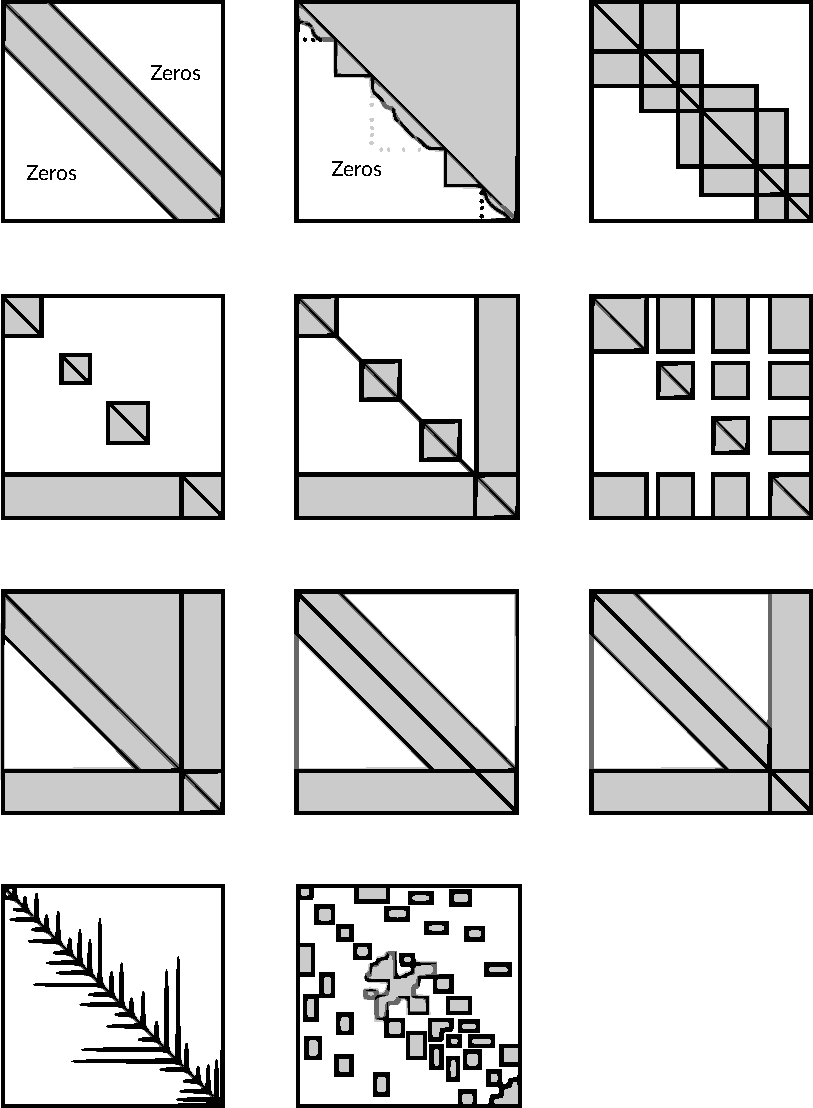
\includegraphics[height=0.8\textheight]{sparse-overview}
  \end{center}
\end{frame}

\section{Laplace's equation}
\subsection*{Laplace's equation}
\againframe<2>{contents_lin3}
\begin{frame}[fragile]
  \frametitle{Laplace's equation}
  \begin{columns}
  \column{0.7\textwidth}
  \begin{align*}
    \frac{\partial T}{\partial t} &= \alpha \nabla^2 T \\
    T &= \text{Temperature} \\
    \alpha &= \text{Thermal diffusivity}
  \end{align*}
  \pause
  \begin{center}
      \begin{tikzpicture}[scale=0.4]
      \draw[black,thick,->] (-0.3,-0.3)-- node[at end,anchor=north]{$x$}(7,-0.3);
      \draw[black,thick,->] (-0.3,-0.3)-- node[at end,anchor=east]{$y$} (-0.3,7);
      \draw[thick,draw=tueorange,fill=tuegreen] (0,0) rectangle +(6,6);
      \node[anchor=west] at (6,3) {$T=T_{b4}$};
      \node[above,anchor=south] at (3,6.5) {$T=T_{b2}$};
      \node[below,anchor=north] at (3,-0.5  ) {$T=T_{b1}$};
      \node[left of=3pt] at (0,3) {$T=T_{b3}$};
%       \node at (0.3,0.3) (A) {};
%       \node at (0.3,5.7) (B) {};
%       \node at (5.7,5.7) (C) {};
%       \node at (5.7,0.3) (D) {};
%       \draw[thick,scharlaken] (A) -- node[midway,anchor=east] {$T=T_{b3}$} (B);
%       \draw[thick,tuegreen] (B) -- node[midway,anchor=south] {$T=T_{b2}$} (C);
%       \draw[thick,tueorange] (C) -- node[midway,anchor=east] {$T=T_{b4}$} (D);
%       \draw[thick,tuegreen] (D) -- node[midway,anchor=south] {$T=T_{b1}$} (A);
      \end{tikzpicture}
    \end{center}
    \pause
  \column{0.3\textwidth}
  In steady state:
  \[
   \nabla^2 T = 0
  \]
  \vskip2em
  \[
   \frac{\partial^2T}{\partial x^2} + \frac{\partial^2T}{\partial y^2} = 0
  \]
\end{columns}
\end{frame}

{\nologo
\begin{frame}[fragile]
  \frametitle{Discretization of Laplace's equation (I)}
  \begin{columns}
  \column{0.6\textwidth}
%     \vskip-2em
    \hspace*{-2em}
    \begin{tikzpicture}[scale=0.75,font=\sffamily\scriptsize]
      \foreach \x in {0,...,5}
        \foreach \y in {0,...,5} 
          {
    %        \pgfmathtruncatemacro{\label}{\x - 5 *  \y +21}
          \ifthenelse{\x=0 \OR \x=5 \OR \y=0 \OR \y=5}{\node [gdot,fill=scharlaken]  (\x\y) at (1.5*\x,1.5*\y) {};}
          \node [gdot,fill=tuesteel]  (\x\y) at (1.5*\x,1.5*\y) {};} 

        \foreach \x [count=\xi] in {0,...,4}
          \foreach \y [count=\yi] in {0,...,4}  
            \draw (\x\y)--(\x\yi)-- (\xi\yi)--(\xi\y)--(\x\y);% (\y\x)--(\yi\x) ;
        
        \onslide<2->{
	  \node[anchor=east] at (00.west) {$j=0$};
	  \node[anchor=east] at (01.west) {$j=1$};
	  \node[anchor=east] at (02.west) {$j=2$};
	  \node[anchor=east] at (04.west) {$j=N_y-2$};
	  \node[anchor=east] at (05.west) {$j=N_y-1$};
	  \node[anchor=north] at (00.south) {$i=0$};
	  \node[anchor=north] at (10.south) {$i=1$};
	  \node[anchor=north] at (20.south) {$i=2$};
	  \node[anchor=north] at (40.south) {$i=N_x-2$};
	  \node[anchor=north west] at (50.south) {$i=N_x-1$};
	}
	
	\onslide<3->{
	  \node[anchor=south west] at (00.north east) {$T_0$};
	  \node[anchor=south west] at (10.north east) {$T_1$};
	  \node[anchor=south west] at (20.north east) {$T_2$};
	  \node[anchor=south west] at (30.north east) {$T_3$};
	  \node[anchor=south west] at (40.north east) {$T_4$};
	  \node[anchor=south west] at (50.north east) {$T_5$};
	  \node[anchor=south west] at (01.north east) {$T_{N_x}$};
	  \node[anchor=south west] at (11.north east) {$T_{N_x+1}$};
	  \node[anchor=south west] at (21.north east) {$T_{N_x+2}$};
	  \node[anchor=south west] at (51.north east) {$T_{2N_x-1}$};
	  \node[anchor=south]      at (55.north) {$T_{N_y N_x - 1} \equiv T_{N_{\mathrm{tot}}}$};
	}
      \end{tikzpicture}
%     \end{center}
  \hfill
  \column{0.35\textwidth}
  \begin{itemize}
    \item<1-> Define a grid of points in $x$ and $y$
    \item<2-> Index of the grid points using 2D coordinates $i$ and $j$
    \item<3> Set up the equations using a 1D index system: $T_{i,j} \rightarrow T_{i + j Nx}$
  \end{itemize}
  \end{columns}
\end{frame}
}

\begin{frame}[fragile]
  \frametitle{Discretization of Laplace's equation (II)}
  Estimate the second-order differentials: assume a piece-wise linear profile in the temperature: \vskip1em
  \begin{columns}
  \column{0.5\textwidth}
    \begin{tikzpicture}[scale=0.7,node distance=5mm]
      \draw[black,thick,->] (0,0)-- node[at end,anchor=north]{$x$}(7,0);
      \draw[black,thick,->] (0,0)-- node[at end,anchor=east ]{$T$}(0,5);
      \node [gdot,fill=scharlaken] (n1) at (1,0) {};
      \node [gdot,fill=scharlaken] (n2) at (3,0) {};
      \node [gdot,fill=scharlaken] (n3) at (5,0) {};
      \node [anchor=south,dot,color=black,fill=black] (e1) at (1,1) {};
      \node [anchor=south,dot,color=black,fill=black] (e2) at (3,2) {};
      \node [anchor=south,dot,color=black,fill=black] (e3) at (5,4) {};
      \node [below=1mm of e1.center,anchor=north west] (e4) {$T_{i-1}$};
      \node [below=1mm of e2.center, anchor=north west] (e5) {$T_{i}$};
      \node [below=1mm of e3.center,anchor=north west] (e6) {$T_{i+1}$};
      \draw[black,thick] (e1.center) -- (e2.center) -- (e3.center);
      \draw[black,thick,<->] (1,-0.5) -- node[midway, below] {$\Delta x$} (2.9,-0.5);
      \draw[black,thick,<->] (3.1,-0.5) -- node[midway, below] {$\Delta x$} (5,-0.5);
      \end{tikzpicture}
%     \end{center}
  \hfill
  \column{0.35\textwidth}
  \pause
  \begin{align*}
    \frac{\partial^2T}{\partial x^2} \approx \frac{\left.\frac{\partial T}{\partial x}\right|_{i+\frac{1}{2}}-\left.\frac{\partial T}{\partial x}\right|_{i-\frac{1}{2}}}{\Delta x} \\[15pt]
    \approx \frac{ \frac{\left(T_{i+1,j}-T_{i,j}\right)}{\Delta x} - \frac{\left(T_{i,j}-T_{i-1,j}\right)}{\Delta x}}{\Delta x}\\[15pt]
    = \frac{T_{i+1,j}-2T_{i,j}+T_{i-1,j}}{(\Delta x)^2}
  \end{align*}
  \end{columns}
\end{frame}

\begin{frame}[fragile]
  \frametitle{Discretization of Laplace's equation (III)}
  The $y$-direction is derived analogously, so that the 2D Laplace's equation is discretized as:
  \[
    \frac{T_{i+1,j}-2T_{i,j}+T_{i-1,j}}{(\Delta x)^2} + \frac{T_{i,j+1}-2T_{i,j}+T_{i,j-1}}{(\Delta y)^2} = 0
  \]
  \pause
  Use a single index counter ${k=i+N_x(j-1)}$, so that the equation becomes:
  \[
    \frac{T_{k+1}-2T_k+T_{k-1}}{(\Delta x)^2} + \frac{T_{k+N_x}-2T_k+T_{k-N_x}}{(\Delta y)^2} = 0
  \]
  \pause
  For an equal spaced grid $\Delta x = \Delta y = 1$:
  \tikz{\node[emphblock, text width=\textwidth,]{\[
   T_{k-N_x} + T_{k-1} - 4T_k + T_{k+1} + T_{k+N_x} = 0
   \]
   \[
      \Rightarrow AT=b
   \]\vskip1ex
   %\Rightarrow T_k = \frac{T_{k-N_x} + T_{k-1} + T_{k+1} + T_{k+N_x}}{4}
  };}
\end{frame}

\section{Creating a sparse system}
\subsection*{A sparse matrix}
\againframe<2>{contents_lin3}
{\nologo
\begin{frame}[fragile]
  \frametitle{Creating the linear system}
  \vskip-1em
  \[
   T_{k-N_x} + T_{k-1} - 4T_k + T_{k+1} + T_{k+N_x} = 0
  \]
  Create a \emph{banded} matrix $A$: the main diagonal $k$ contains -4, whereas the bands at $k-1$, $k+1$, $k-N_x$ and $k+N_x$ contain a 1. Boundary cells just contain a 1 on the main diagonal so that the temperature is equal to $T_b$ (e.g. $T_1 = 1T_b$).\\
  \vskip1em
  \hspace*{8em}
  ${
    \begin{bmatrix}
      1 & 0 & 0 & 0 & 0 & 0 & 0 & 0 & \cdots & 0\\
      0 & 1 & 0 & 0 & 0 & 0 & 0 & 0 & \cdots & 0\\
    \vdots & \vdots & \vdots & \vdots & \vdots & \vdots & \vdots & \vdots & \ddots & \vdots\\
     \cdots & 1 & \cdots & 1 & -4 & 1 &\cdots & 1 & \ddots & 0\\
     0 & \cdots & 1 & \cdots & 1 & -4 & 1 &\cdots & 1 & \vdots\\
     \vdots & \vdots & \vdots & \vdots & \vdots & \vdots & \vdots & \vdots & \ddots & \vdots\\
     0 & 0 & 0 & 0 & 0 & 0 & 0 & 0 & 1 & 0\\
     0 & 0 & 0 & 0 & 0 & 0 & 0 & 0 & 0 & 1\\
    \end{bmatrix}
    \begin{bmatrix}
    T_0\\
    T_1\\
    \vdots\\
    T_k\\
    T_k+1\\
    \vdots\\
    T_{N_y N_x - 2}\\
    T_{ N_y N_x - 1}
   \end{bmatrix} = 
   \begin{bmatrix}
    T_b\\
    T_b\\
    \vdots\\
    0\\
    0\\
    \vdots\\
    T_b\\
    T_b
   \end{bmatrix}}$
\end{frame}
}

\begin{frame}[fragile]
  \frametitle{Creating the linear system}
  \vskip-1em
  \[
   T_{k-N_x} + T_{k-1} - 4T_k + T_{k+1} + T_{k+N_x} = 0
  \]
  Create a \emph{banded} matrix \(A\) in Python, by setting the coefficients for the internal cells:
\begin{lstlisting}
import numpy as np
from scipy.sparse import diags

Nx,Ny = 50,50 # Number of grid points along x,y direction
Nc = Nx*Ny    # Total number of points

e = np.ones(Nc)
A = diags([e, e, -4*e, e, e], [-Nx, -1, 0, 1, Nx], shape=(Nc,Nc))
b = np.zeros(Nc)
\end{lstlisting}
The function \lstinline$diags$ uses the following arguments:
\begin{itemize}
   \item The coefficients that have to be put on the diagonals arranged as columns in a matrix
   \item The position of the bands with respect to the main diagonal
   \item Size of the resulting matrix (in our case square $N_xN_y \times N_xN_y$)
  \end{itemize}
\end{frame}

\begin{frame}[fragile]
  \frametitle{Matrix sparsity}
  \begin{columns}
  \column{0.5\textwidth}
  
  \begin{itemize}
   \item Let's check the matrix layout by adding:
   \begin{lstlisting}
print(A)
plt.spy(A, marker='o',markersize=6)
   \end{lstlisting}
    \item The \emph{sparse} structure stores/prints only the nonzero elements
    \item \lstinline|spy| shows the location of the nonzero values in the matrix
    \item Apart from the main diagonal, there are offset bands!
  \end{itemize}
  \column{0.5\textwidth}
    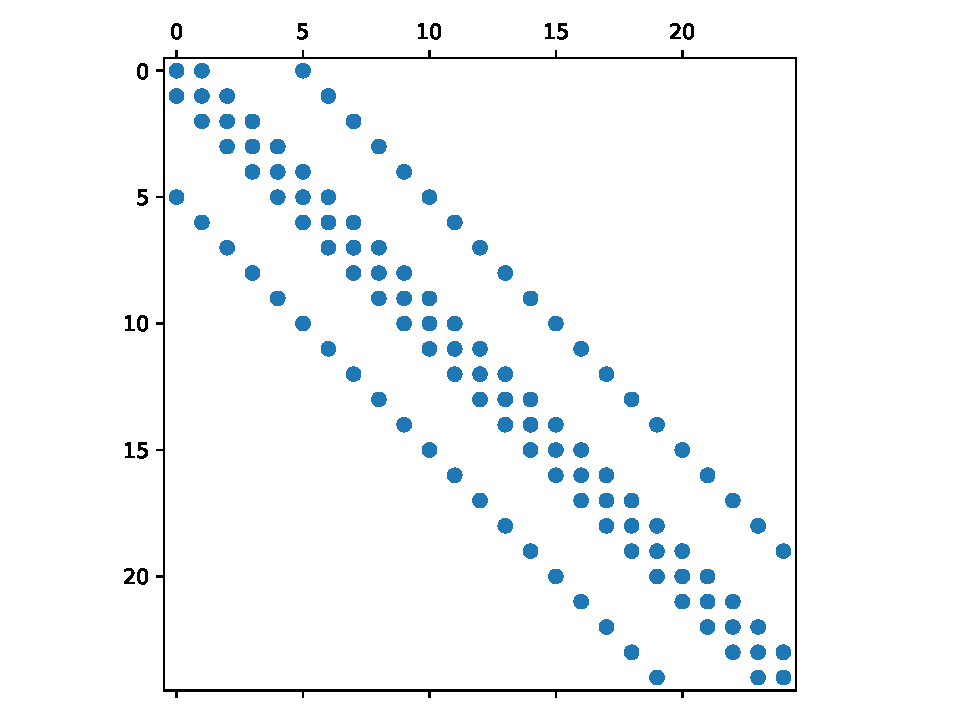
\includegraphics[width=\columnwidth]{sparse_python}
  \end{columns}
\end{frame}

\subsection*{Boundary conditions}
\begin{frame}[fragile]
  \frametitle{About boundary conditions}
  \begin{itemize}
    \item For the nodes on the boundary, we have a simple equation:
    \[
      T_{k,\text{boundary}} = \text{Some fixed value}
      \]
      \item However, we have set all nodes to be a function of their neighbors 
      \item Solution: Determine the boundary node indices $k$ and set the coefficients accordingly
      \begin{lstlisting}
bnd_bottom = np.arange(Nx)
bnd_left = np.arange(Ny) * Nx
bnd_right = bnd_left + Nx - 1
bnd_top = bnd_bottom + Nx*(Ny-1)
      \end{lstlisting}
      \item Reset each row $k$ in $A$ to zeros, then set element $A_{kk} = 1$
      \item Set values in rhs: $b_k = T_{\text{boundary}}$
      \item Boundary conditions are often more elaborate to implement!
  \end{itemize}
\end{frame}

{\nologo
\begin{frame}[fragile]
  \frametitle{Implementation of the boundary conditions}
  A (shortened) version of the \lstinline|set_boundary_conditions(A,b,Tb,Nx,Ny)| function:
  \begin{lstlisting}[language=Python]
def set_boundary_conditions(A, b, Tb, Nx, Ny):

    A = lil_matrix(A) # Required for efficient modification of the sparsity

    # Select nodes that lie at the boundaries
    bnd_bottom = np.arange(Nx)
    bnd_left = np.arange(Ny) * Nx
    bnd_right = bnd_left + Nx - 1
    bnd_top = bnd_bottom + Nx*(Ny-1)

    bnd_all = np.unique(np.concatenate((bnd_bottom,bnd_left,bnd_right,bnd_top)))

    # Reset the coefficient row to zero, add a 1 only on the main diagonal
    A[bnd_all,:] = 0
    A[bnd_all,bnd_all] = 1

    b[bnd_bottom] = Tb['bottom']
    b[bnd_left] = Tb['left']
    b[bnd_right] = Tb['right']
    b[bnd_top] = Tb['top']

    return A.tocsr(), b
  \end{lstlisting}
\end{frame}
}

\begin{frame}[fragile]
  \frametitle{How applying boundary conditions affects the linear system}
  Using the functions provided in \lstinline|laplace_demo.py|:
  \begin{lstlisting}[language=Python]
Nx = Ny = 5 # number of internal grid cells over x/y-direction

T_boundary = {'bottom': 300, 'left': 1000, 'right': 1000, 'top': 500}

A,b = create_laplace_coefficient_matrix(Nx,Ny)
A,b = set_boundary_conditions(A, b, T_boundary, Nx, Ny)  
  \end{lstlisting}
  \pause
  \begin{columns}[T]
    \column{0.5\textwidth}
    Check the new structure of the matrix and the right hand side:
      \begin{lstlisting}
  plt.subplot(121); plt.spy(A2);
  plt.subplot(122); plt.spy(b[:,None]);
      \end{lstlisting}
    \column{0.5\textwidth}
    \centering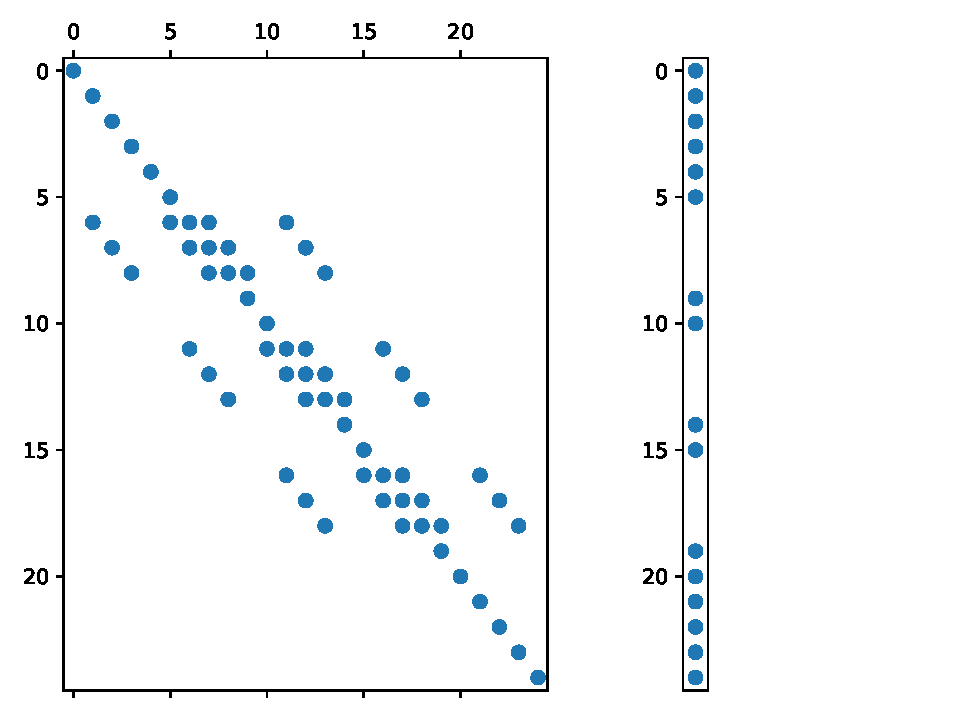
\includegraphics[width=0.8\columnwidth]{sparse_python_bnds}
  \end{columns}
\end{frame}

\subsection*{Solving the equation}
\begin{frame}[fragile]
  \frametitle{A full program, including solver}
  The program and auxiliary functions are on Canvas (\lstinline$laplace_demo.py$)
      \begin{lstlisting}
import numpy as np
from scipy.sparse.linalg import spsolve
from matplotlib import cm
import matplotlib.pyplot as plt

Nx = Ny = 20

T_boundary = {'bottom': 300, 'left': 1000, 'right': 1000, 'top': 500}

A,b = create_laplace_coefficient_matrix(Nx,Ny)
A,b = set_boundary_conditions(A, b, T_boundary, Nx, Ny)

T = spsolve(A,b).reshape((Nx,Ny))

fig, ax = plt.subplots(subplot_kw={"projection": "3d"})
x,y = np.meshgrid(np.arange(Nx),np.arange(Ny))
surf = ax.plot_surface(x,y,T,cmap=cm.inferno)
fig.colorbar(surf, shrink=0.5)
plt.show()
      \end{lstlisting}
\end{frame}

  
\begin{frame}[fragile]
  \frametitle{Sample results}
  \begin{center}
    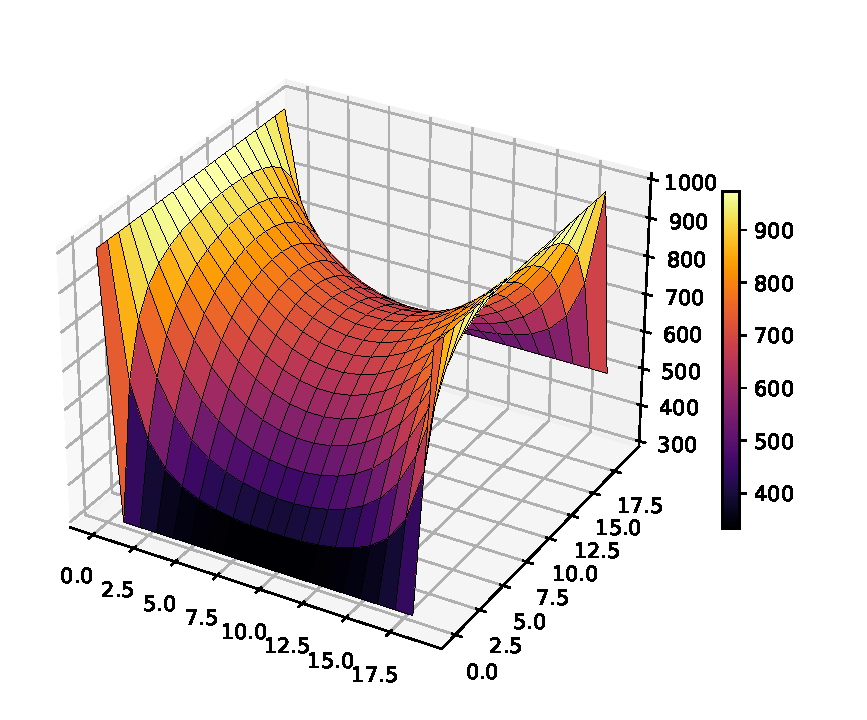
\includegraphics[width=0.65\textwidth]{laplace_20x20}
  \end{center}
\end{frame}

{\nologo
\begin{frame}[fragile]
  \frametitle{Exercise: Verify the numerical solution using Fourier-series}
  A Fourier-series expansion for the steady-state heat conduction in a flat plate is given for a domain: $x,y\in[0,1]$ , with fixed-temperature boundaries $T\big|_{x=0} = T\big|_{x=1} = T\big|_{y=0}=0$ and $T\big|_{y=1}=1$:
\[
    T = \frac{4}{\pi} \sum_{n=1}^\infty \frac{\sin\left(m \pi x \right)\sinh\left(m\pi y \right)}{m \sinh\left(m \pi \right)} \quad \text{with} \quad m=2n-1
\]
Compute and plot the exact temperature profile in the 2D plate, and compare it with the numerical solution:
  \begin{hints}
  Hints:
  \begin{itemize}
      \item Use meshgrid to create a mesh in $x$ and $y$
      \item Compute the temperature using the Fourier series, use vectorised computations over $x$ and $y$ so that only 1 loop (over n) is required.
      \item Solve the numerics for the same problem (note the boundary conditions)
      \item Compare the numerical and exact solutions (e.g. a plot).
  \end{itemize}
  \end{hints}
\end{frame}

\begin{frame}<beamer:1-|handout:0>[fragile]
  \frametitle{Exercise: Verify the numerical solution using Fourier-series}
  Full script in \lstinline{solveLaplaceEqAndFourier.py}
    \begin{lstlisting}
import numpy as np
import matplotlib.pyplot as plt
import matplotlib.cm as cm

Nx = Ny = 20

xf,yf = np.meshgrid(np.linspace(0,1,Nx),np.linspace(0,1,Ny))
term = np.zeros_like(x)
N = 100

for m in range(1,N,2):
    term = term + (np.sin(m*np.pi*xf)*np.sinh(m*np.pi*yf)) / (m*np.sinh(m*np.pi))

sol = term * 4 / np.pi
fig, ax = plt.subplots(subplot_kw={"projection": "3d"})
surf = ax.plot_surface(x,y,sol,cmap=cm.inferno)
fig.colorbar(surf, shrink=0.5)
plt.show()
    \end{lstlisting}
\end{frame}
}

\begin{frame}[fragile]
  \frametitle{LU decomposition of a sparse matrix}
  \begin{columns}
  \column{0.35\textwidth}
    \begin{lstlisting}[basicstyle=\ttfamily\tiny]
import numpy as np
from scipy.linalg import lu
import matplotlib.pyplot as plt
from laplace_demo import create_laplace_coefficient_matrix

A,b = create_laplace_coefficient_matrix(5,5)

# Perform LU decomposition
# Note: lu does not work on sparse arrays,
# so we map to a full array
P,L,U = lu(A.toarray())

# Plot the sparsity patterns of L and U
plt.subplot(121)
plt.spy(L)
plt.title('L')
plt.subplot(122)
plt.spy(U)
plt.title('U')
plt.tight_layout()
    \end{lstlisting}
  \column{0.65\textwidth}
  \pause
  \begin{itemize}
    \item With LU decomposition we produce matrices that are less sparse than the original matrix.
    \item Sparse storage often required, and also numerical techniques that fully utilizes this!
  \end{itemize}\vskip2em
  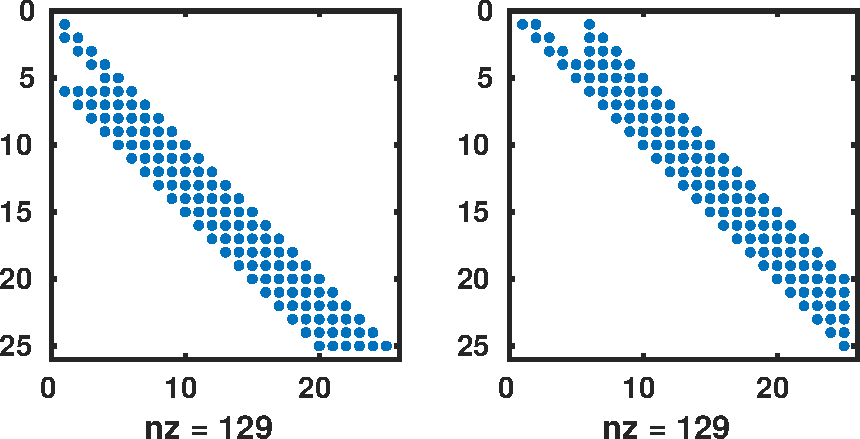
\includegraphics[width=\columnwidth]{sparse_lu}
  \end{columns}
\end{frame}
  
\begin{frame}[fragile]
  \frametitle{LU decomposition}
  \begin{itemize}
    \item LU decomposition and Gaussian elimination on a matrix like $A$ requires more memory (with 3D problems, the offset in the diagonal would even be bigger!)
    \item In general extra memory allocation will not be a problem for Python
    \item Python is clever, in that sense that it attempts to reorder equations, to move elements closer to the diagonal)
  \end{itemize} \pause
  Alternatives for elimination methods
  \begin{itemize}
    \item Use iterative methods when systems are large and sparse.
    \item Often such systems are encountered when we want to solve PDE’s of higher dimensions
  \end{itemize}
\end{frame}

\section{Iterative methods}
\subsection*{Introduction}
\againframe<2>{contents_lin3}

\begin{frame}[fragile]
  \frametitle{Examples of iterative methods}
  \begin{itemize}
    \item Jacobi method
    \item Gauss-Seidel method
    \item Succesive over relaxation \vskip2em
    \item \lstinline$bicg$ --- Bi-conjugate gradient method
  \item \lstinline$pcg$ --- preconditioned conjugate gradient method
  \item \lstinline$gmres$ --- generalized minimum residuals method
  \item \lstinline$bicgstab$ --- Bi-conjugate gradient method
\end{itemize}
\end{frame}

\subsection*{Jacobi method}
\begin{frame}[fragile]
  \frametitle{The Jacobi method}
  \begin{itemize}
     \item In our example we derived the following equation:
    \[
     T_{k-N_x} + T_{k-1} - 4T_k + T_{k+1} + T_{k+N_x} = 0
    \]
    \item Rearranging gives:
    \[
      T_k = \frac{T_{k-N_x} + T_{k-1} + T_{k+1} + T_{k+N_x}}{4}
    \]\pause
    \item In the Jacobi scheme the iteration proceeds as follows:
    \begin{enumerate}
      \setlength{\itemindent}{1cm}
      \item Start with an initial guess for the values of $T$ at each node\pause
      \item Compute updated values and store a new vector:
        \[
          T_k^\text{new} = \frac{T_{k-N_x}^\text{old} + T_{k-1}^\text{old} + T_{k+1}^\text{old} + T_{k+N_x}^\text{old}}{4}
        \]\pause
      \item Do this for all nodes\pause
      \item Repeat the procedure until converged
    \end{enumerate}
  \end{itemize}
\end{frame}

\begin{frame}[fragile]
  \frametitle{Jacobi method for Laplace's equation}
  \vskip-1em
  See \lstinline$laplace_jacobi.py$ for animation included (from Canvas)
  \begin{columns}
    \column{0.35\textwidth}
    \begin{lstlisting}[]
import numpy as np
import matplotlib.pyplot as plt

# Set grid resolution
nx = 40
ny = 40

# Set old solution array
T = np.zeros((nx,ny))

# Set boundary conditions
T[0,:] = 40 # Left
T[nx-1,:] = 60 # Right
T[:,0] = 20 # Bottom
T[:,ny-1] = 30 # Top

# Set new solution array (inc bnd conditions)
Tnew = T.copy()
    \end{lstlisting}      
    \column{0.65\textwidth}
  \begin{lstlisting}[]
# Create grid for plotting
x,y = np.meshgrid(np.arange(1,nx+1), np.arange(1,ny+1))

# Perform iterations
for iter in range(1,1001):
    for i in range(1,nx-1):
        for j in range(1,ny-1):
            # Calculate new solution
            Tnew[i,j] =  \
                (T[i-1,j]+T[i+1,j]+T[i,j-1]+T[i,j+1])/4.0 
    T = Tnew.copy()
    \end{lstlisting}
    \pause
    $\rightarrow$ Try to modify this script so that 1 cell/block of cells in the center is kept at 100 degrees
  \end{columns}
\end{frame}

\begin{frame}[fragile]
  \frametitle{About the straightforward implementation}
  \begin{itemize}
  
   \item The method as implemented works fine for a simple Laplace equation
%    \item We did not take into account the thermal diffusivity (set to unity)
%    \item We did not take into account the grid spacing (set to unity)
   \item For generic systems of linear equations, the implementation cannot be used.
  \end{itemize}\vskip2em\pause
 \tikz{\node[emphblock,text width=\textwidth]{We will now introduce the Jacobi method so it can be used for generic systems of linear equations.};}
\end{frame}

\begin{frame}[fragile]
  \frametitle{The Jacobi method with matrices}
  We can split our (banded) matrix $A$ into a diagonal matrix $D$ and a remainder $R$:\vskip1em
  \[
   A \quad =\quad  D \quad + \quad R
  \]
 \vskip2em
  \scalebox{0.6}{
  $
   \begin{bmatrix}
    \times & \times &  &  &  &  & \times &  & \\
    \times & \times & \times &   &   &   &   & \times &    \\
           & \times & \times & \times &   &   &   &   & \times \\
           &   & \times & \times & \times &   &   &   &   \\
      &   &   & \times & \times & \times &   &   &    \\
      &   &   &   & \times & \times & \times &   &   \\
      \times &   & &   &   & \times & \times & \times &   \\
      &   \times &   & &   &   & \times & \times & \times \\
      &   &   \times &   & &   &   & \times & \times \\
   \end{bmatrix} = 
   \begin{bmatrix}
    \times &  &  &  &  &  &  &  & \\
     & \times &  &   &   &   &   &  &    \\
           &  & \times &  &   &   &   &   &  \\
           &   &  & \times &  &   &   &   &   \\
     &   &   &  & \times &  &   &   &    \\
      &  &   &   &  & \times &  &   &   \\
      &   &  &   &   &  & \times &  &   \\
      &   &   &  &   &   &  & \times &  \\
      &   &   &   &  &   &   &  & \times \\
   \end{bmatrix} + 
   \begin{bmatrix}
     & \times &  &  &  &  & \times &  & \\
    \times &  & \times &   &   &   &   & \times &    \\
           & \times &  & \times &   &   &   &   & \times \\
           &   & \times &  & \times &   &   &   &   \\
      &   &   & \times &  & \times &   &   &    \\
      &   &   &   & \times &  & \times &   &   \\
      \times &   & &   &   & \times &  & \times &   \\
      &   \times &   & &   &   & \times &  & \times \\
      &   &   \times &   & &   &   & \times &  \\
   \end{bmatrix}$}
\end{frame}

\begin{frame}[fragile]
  \frametitle{Jacobi method: solving a system}
  \begin{itemize}
   \item We can solve $AT=b$, now written generally as $Ax=b$, by:
   \begin{align*}
      Ax&=b\\
     (D+R)x &= b \\
      Dx &= b -Rx \\
      Dx^\text{new} &= b - Rx^\text{old} \\
       x^\text{new} &= D^{-1}(b-Rx^\text{old})
   \end{align*}
   \item Using the $n$ and $n+1$ notation for old and new time steps, we find in general:
   \[
    x^{n+1} = D^{-1}\left(  b-Rx^n\right)
   \]
   \[
    x_i^{n+1} = \frac{1}{A_{ii}}\left(b_i - \sum_{j\neq i} A_{ij}x_j^n\right)
   \]
  \end{itemize}
\end{frame}

\begin{frame}[fragile]
  \frametitle{Diagram of the Jacobi method}
  \begin{tikzpicture}[scale=0.5,font=\tiny,node distance = 25pt, auto,->=stealth,point/.style={circle,fill=red,minimum size=0pt,inner sep=0pt}]
    \tikzstyle{block2} = [rectangle,minimum height=1em,draw=maincolor,fill=maincolor!20,text centered,rounded corners,minimum height=2em,thick,text width=1.5cm]
    \node[block2]                 (start) {Set $T^\text{old}$ = a guess};
    \node[block2, right=of start,visible on=<2->] (calc)  {Calculate the new node solution with previous values.};
    \node[block2, right=of calc,visible on=<3->] (check1) {Have all nodes been updated?};
    \node[block2, right=of check1,,visible on=<5->,text width=2cm] (tol) {Tolerance check: $\frac{\mynorm{Ax-b}_2}{\mynorm{b}_2} \leq \text{tol} $?};
    \node[block2, above=of check1,visible on=<4->] (next) {Move to next node};
    \node[block2, above=of tol,visible on=<6->] (update) {Update $T^\text{old}=T^\text{new}$};
    \node[block2, below=of tol,visible on=<8->] (answer) {Report the answer as $T^\text{new}$};
    \draw[->,thick,black,visible on=<2->] (start.east) -- (calc.west);
    \draw[->,thick,black,visible on=<3->] (calc.east) -- (check1.west);
    \draw[->,thick,black,visible on=<5->] (check1.east) -- node[midway,above]{Yes} (tol.west);
    \draw[->,thick,black,visible on=<4->] (check1.north) -- node[midway]{No} (next.south);
    \draw[->,thick,black,visible on=<6->] (tol.north) -- node[midway,left] {No} (update.south);
    \draw[->,thick,black,visible on=<8->] (tol.south) -- node[midway,left] {Yes} (answer.north);
    \draw[->,thick,black,visible on=<7->] (update.north) |- ++(0,0.5cm) -| ($ (calc.north) + (-5mm,0)$);
    \draw[->,thick,black,visible on=<4->] (next.west) -| ($ (calc.north) + (5mm,0)$);
    
%     \draw[->,thick,black] (tol.north) -| ($ (digit.east) + (2mm,0) $) (calc.west);
%     \draw[->,thick,black] (start.east) -- (calc.west);
  \end{tikzpicture}
\end{frame}

\begin{frame}[fragile]
  \frametitle{The core of the solver}
  The full function \lstinline|jacobi(A, b, tol=1e-2)| is on Canvas, see \lstinline$it_methods.py$. The gist is:
  \begin{lstlisting}[numbers=left]
# While not converged or max_it not reached
while (x_diff > tol and it_jac < 1000):
    x_old = x.copy()
    for i in range(N):
        s = 0
        for j in range(N):
            if j != i:
                # Sum off-diagonal*x_old
                s += A[i,j] * x_old[j]
        # Compute new x value
        x[i] = (b[i] - s) / A[i,i]
        
    # Increase number of iterations
    it_jac += 1
    x_diff = norm(A@x - b)/norm(b)
  \end{lstlisting}
  \pause
  Try to call it from the \lstinline$laplace_demo.py$ file, instead of using \lstinline$spsolve$.
\end{frame}

\begin{frame}[fragile]
  \frametitle{A few details on this algorithm}
  \begin{itemize}
   \item The while loop holds two aspects
   \begin{itemize}
    \item A convergence criterion (\lstinline$norm(A@x - b)/norm(b) > tol$). Some considerations are:
    \begin{itemize}
      \item $L_1$-norm (sum)
      \item $L_2$-norm (Euclidian distance)
      \item $L_\infty$-norm (max)
    \end{itemize}
    \item Protection against infinite loops (no convergence)
   \end{itemize}\pause
   \item Reset the sum for each row, before summing for the new unknown node
  \end{itemize}\pause
  \vskip1em
  \begin{itemize}
    \item Start vector x is not shown in the example, but should be there!
    \item It can have huge impact on performance!
    \item The for-loops also have a large performance penalty!
  \end{itemize}
\end{frame}

\begin{frame}[fragile]
  \frametitle{The solver using array indices}
  Make a copy of the Jacobian solver, and replace the for-loop on \lstinline|j| by a vector-operation in a new function \lstinline|jacobi_vec(A, b, tol=1e-2)|:
  \begin{onlyenv}<beamer>
  \begin{lstlisting}[basicstyle=\scriptsize\ttfamily]
# While not converged or max_it not reached
while (x_diff > tol and it_jac < 1000):
    x_old = x.copy()
    for i in range(N):
        j = np.r_[np.arange(i),np.arange(i+1,N)]
        # Sum off-diagonal*x_old
        s = A[i,j] @ x_old[j]
        # Compute new x value
        x[i] = (b[i] - s) / A[i,i]
        
    # Increase number of iterations
    it_jac += 1
    x_diff = norm(A@x - b)/norm(b)
    \end{lstlisting}
  \end{onlyenv}
\end{frame}

\begin{frame}[fragile]
  \frametitle{Iterations 1, 2, 5 and 10}
  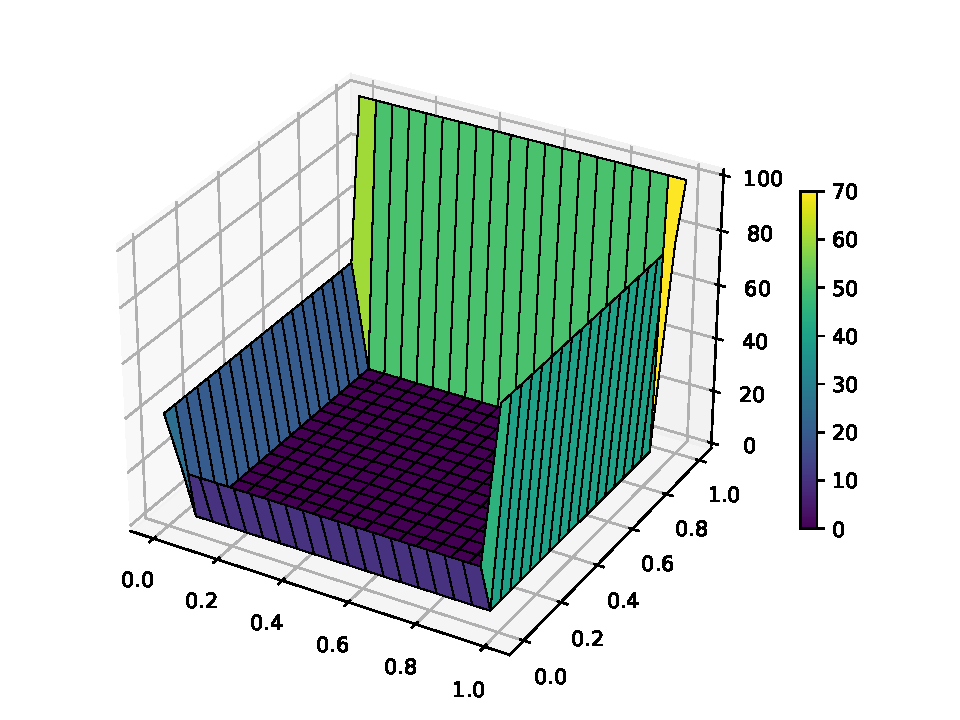
\includegraphics[width=0.35\textwidth]{python_it1.pdf} \hspace{0.5cm}
  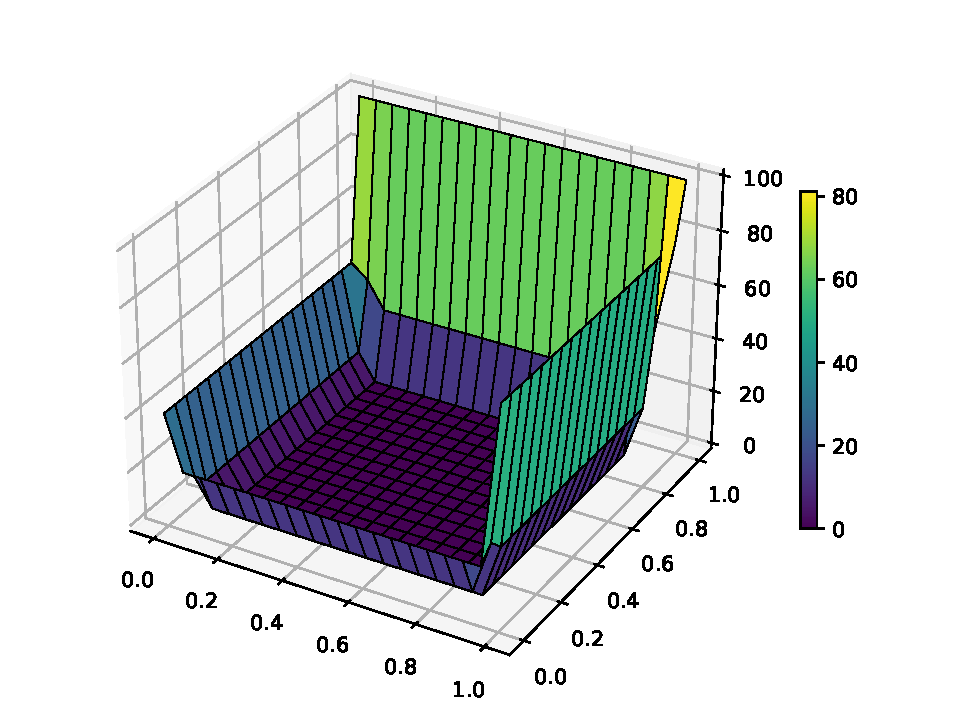
\includegraphics[width=0.35\textwidth]{python_it2.pdf}\\
  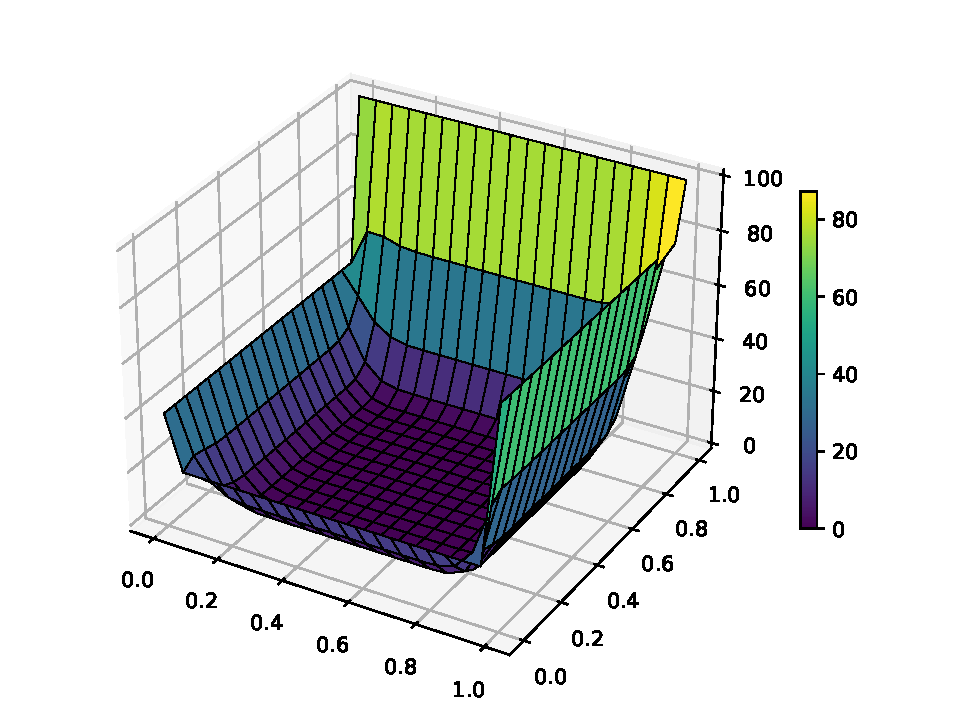
\includegraphics[width=0.35\textwidth]{python_it5.pdf} \hspace{0.5cm} 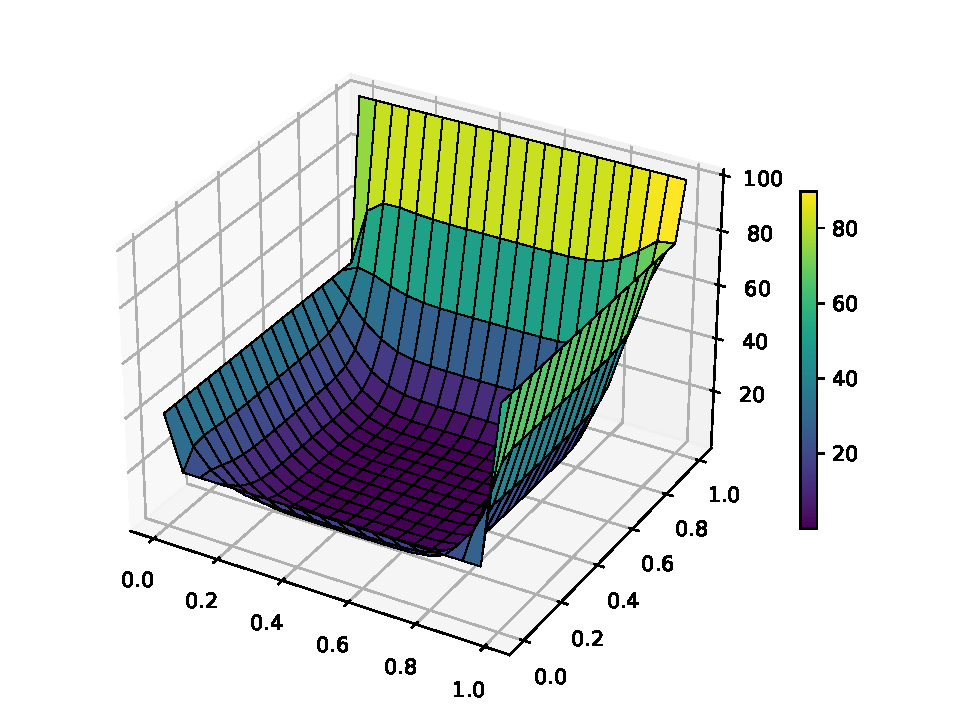
\includegraphics[width=0.35\textwidth]{python_it10.pdf}
\end{frame}

\subsection*{Gauss-Seidel method}
\begin{frame}[fragile]
  \frametitle{Gauss-Seidel method}
  The Gauss-Seidel method is quite similar to Jacobi method
  \begin{itemize}
   \item The only difference is that the new estimate $x^\text{new}$ is returned to the solution $x^\text{old}$ as soon as it is completed
   \item For following nodes, the updated solution is used immediately \pause
   \item Our straightforward script (from the Jacobi method) is therefore changed easily:
   \begin{itemize}
    \item Do not create a \lstinline$Tnew$ array (save memory!)
    \item Do not store the solution in \lstinline$Tnew$, but simply in \lstinline$T$
    \item Do not perform the update step \lstinline$T=Tnew$
    \item See \lstinline$gaussseidel(A, b, tol=1e-2)$ for the algorithm.\pause
   \end{itemize}
   \item The straightforward script works well for the current Laplace equation, but we define the generic Gauss-Seidel algorithm on the following slides.
  \end{itemize}
\end{frame}

\begin{frame}[fragile]
  \frametitle{Gauss-Seidel method}
  \begin{itemize}
    \item Define a lower and strictly upper triangular matrix, such that $A = L + U$
    \item Now we can solve AT=b by:
    \begin{align*}
      (L+U)T &= b \\
      LT &= b - UT \\
      LT^\text{new} &= b - UT^\text{old} \\
      T^\text{new} &= L^{-1}(b-UT^\text{old})
   \end{align*}
     \item Using the $n$ and $n+1$ notation for old and new time steps, we find in for the general Gauss-Seidel method:
     \[
      x^{n+1} = L^{-1}\left(b-Ux^n\right)
     \]
     \[
      x_i^{n+1} = \frac{1}{A_{ii}}\left(b_i - \sum_{j<i} A_{ij}x_j^{n+1}- \sum_{j>i} A_{ij}x_j^n\right)
     \]
  \end{itemize}
\end{frame}

\begin{frame}[fragile]
  \frametitle{Create yourself: Gauss-Seidel method}
  \begin{itemize}
    \item Create a copy of the \lstinline|jacobi| method and rename it to \lstinline|gaussseidel|
    \item Rework the inner algorithm to reflect the changes for the Gauss-Seidel method
    \item Test! Perform a timing check and check if the solution is correct.
    \item Next, create a new copy of the just created method and vectorize it, analogous to our vectorized Jacobi method
  \end{itemize}
\end{frame}
    
\section{Summary}
\subsection*{Summary}
\againframe<2>{contents_lin3}
\begin{frame}[fragile]
  \frametitle{Summary}
  \begin{itemize}
    \item Partial differential equations can be discretized into sparse systems of linear equations
    \item Sparse matrices can be stored in memory efficiently using specialised formats (e.g. compressed row storage)
    \item The Jacobi and Gauss–Seidel methods were introduced as iterative methods; other methods are based on the same principle (successive over-relaxation method, for example)
    \item Various implementation issues were discussed, e.g. vectorised computing, convergence tolerances
  \end{itemize}
\end{frame}

\begin{frame}[fragile]
  \frametitle{Direct methods vs. Iterative methods}
  \begin{itemize}
    \item Iterative methods converge \emph{gradually} to a solution while direct methods (possibly with partial pivoting) factorise a (set of) matrix(ces) which allow to compute the solution by \emph{substitution}.
    \item Direct methods generally use more memory, since they need to store also the result matrices.
    \item A strictly (or irreducibly) diagonally dominant matrix is a prerequisite for convergence of the Jacobi and Gauss-Seidel method.
    \item For real-life situations; 1D problems are generally solved with direct methods (LU decomposition). If you have systems of more than 1 dimension, a direct method still can be used, if there are no memory issues, otherwise an iterative method would be more attractive.
\end{itemize}
\end{frame}